\documentclass[12pt,titlepage]{article}
\usepackage{geometry}

\usepackage[utf8]{inputenc}
\usepackage[greek,english]{babel}
\usepackage{alphabeta}
\usepackage[T1]{fontenc}

\usepackage{minted}
\usepackage{xcolor}
\usemintedstyle{friendly}
\setminted{breaklines,frame=lines}

\usepackage{booktabs}
\usepackage{csvsimple}

\usepackage{graphicx}
\graphicspath{{../plots/}}

\begin{document}

\title{Συστήματα Παράλληλης Επεξεργασίας\\
    Άσκηση 2}
\author{Αλέξιος Ζαμάνης\\
    03115010\\
    Παναγιώτης Ζώγας\\
    03115191}
\date{\selectlanguage{greek}\today}

\maketitle

\section{Διάδοση θερμότητας σε δύο διαστάσεις}

Στο πλαίσιο αυτής της άσκησης μελετούμε την επίλυση της εξίσωσης Laplace, μιας
τυπικής μερικής διαφορικής εξίσωσης. Συγκεκριμένα αχολούμαστε με την απλούστερη
περίπτωση των δισδιάστατων (επίπεδων) καρτεσιανών συντεταγμένων. Προσεγγίζουμε
την επίλυσή της εξίσωσης με τη μέθοδο Jacobi και δύο παραλλαγές της, τις
Gauss-Seidel SOR και Red-Black SOR, που συγκλίνουν ταχύτερα.

Στόχος μας είναι να παραλληλοποιήσουμε τις υλοποιήσεις των μεθόδων, ώστε να
μπορούν να εκτελεστούν σε συστήματα κατανεμημένης μνήμης με κατανεμημένο χώρο
διευθύνσεων. Ως εκ τούτου, χρησιμοποιούμε το de facto πρότυπο για την υλοποίηση
ανταλλαγής μηνυμάτων, το MPI.

Προφανώς ακολουθούμε μια data centric προσέγγιση. Ήτοι χωρίζουμε τα δεδομένα
αποστέλλοντάς τα στις διαθέσιμες διεργασίες και αυτές στη συνέχεια εκτελούν
τους υπολογισμούς στο κομμάτι που έλαβαν. Στο τέλος μαζεύουμε τα αποτελέσματα
από τις επιμέρους διεργασίες και συνθέτοντάς τα προκύπτει η συνολική λύση.

Στο MPI η προαναφερθείσα διαδικασία διασκορπισμού και συλλογής των δεδομένων
υλοποιείται χρήσει των συναρτήσεων MPI\_Scatterv και MPI\_Gatherv. Συγκεκριμένα
έχουμε:

\begin{minted}{C}
MPI_Scatterv(rank == 0 ? U[0] : NULL, scattercounts, scatteroffset, global_block, &u_current[1][1], 1, local_block, 0, CART_COMM);
memcpy(u_previous[0], u_current[0], (local[0] + 2) * (local[1] + 2) * sizeof(double));
...
MPI_Gatherv(&u_current[1][1], 1, local_block, rank == 0 ? U[0] : NULL, scattercounts, scatteroffset, global_block, 0, CART_COMM);
\end{minted}

Έχουμε δηλαδή έναν συνολικό πίνακα (U) στην ριζική διεργασία (αυτή που έχει
μηδενικό rank) και δύο μερικούς πίνακες (u\_current και u\_previous) σε κάθε
διεργασία (συμπεριλαμβανομένης της ριζικής). Όλες οι διεργασίες ανήκουν στον
ίδιο communicator, τον CART\_COMM, που αποτελεί ένα mapping του default
communicator, του MPI\_COMM\_WORLD, σε ένα δισδιάστατο πλέγμα.

Έχουν ήδη ορισθεί 2 user-defined data types, τα global\_block και local\_block,
που ορίζουν την έννοια του block στο συνολικό και στους μερικούς πίνακες
αντίστοιχα. Ομοίως, έχουν ορισθεί τα scattercounts και scatteroffset, που
ορίζουν το πλήθος των blocks που θα αποσταλλούν (προφανώς 1) και τη θέση τους
στον U (συναρτήσει της θέσης της διεργασίας στο πλέγμα). Παρακάτω θα ορίσουμε
εμείς data types και θα τα συζητήσουμε εκτενέστερα.

Επομένως με την MPI\_Scatterv η ριζική διεργασία αποστέλλει στις διεργασίες του
CART\_COMM (όλες τις διεργασίες) έναν υποπίνακα (ως global\_block) που βρίσκεται
σε ένα συγκεκριμένο offset από την αρχή του U. Κάθε διεργασία λαμβάνει τον
υποπίνακα (ως local\_block) και τον αποθηκεύει στον u\_current ξεκινώντας από τη
θεση (1, 1), καθώς οι μερικοί πίνακες έχουν 2 παραπάνω στήλες και γραμμές. Έτσι
εν τέλει δημιουργούμε ένα περίγραμμα από ghost cells (θα μας χρειαστούν στη
συνέχεια).

Σημειώνουμε ότι για τις διεργασίες πλην της ριζικής ο U δεν έχει νόημα, οπότε
φροντίζουμε να ορίσουμε σαν source το NULL. Επιπλέον κάθε διεργασία φροντίζει να
αρχικοποιήσει και τον u\_previous, αντιγράφοντάς του τα δεδομένα που έλαβε.
Τέλος σημειώνουμε ότι η MPI\_Gatherv συντάσσεται αντίστοιχα με την MPI\_Scatterv
και εκτελεί την ακριβώς αντίστροφη διαδικασία.

Όλη η προαναφερθείσα διαδικασία συμβαίνει ακριβώς στην αρχή (scatter) και στο
τέλος (gather) της εκτέλεσης. Εδώ ξεχωριστό ρόλο παίζει η διαδικασία που έχει
ορισθεί ως ριζική, καθώς διαμοιράζει το input και συλλέγει το output (στην ουσία
εκτελεί όλο το IO). Στο υπόλοιπο (ενδιάμεσο) πρόγραμμα όλες οι διεργασίες
θεωρούνται πλήρως ισότιμες. Πρόκειται δηλαδή για καθαρό SPMD.

Ωστόσο, οι κατανεμημένοι υπολογισμοί δεν είναι ανεξάρτητοι μεταξύ τους. Μια
διεργασία πρέπει να επικοινωνεί με τους γείτονές της, ώστε να ανταλλάσσουν τις
συνοριακές γραμμές και στήλες τους κάθε φορά που εκτελείται ένας κύκλος
υπολογισμών και ενημερώνονται οι τιμές τους.

Ως εκ τούτου, οφείλουμε να ορίσουμε τύπους δεδομένων για τις γραμμές και τις
στήλες. Έχουμε:

\begin{minted}{C}
MPI_Datatype local_row;
MPI_Type_contiguous(local[1], MPI_DOUBLE, &dummy);
MPI_Type_create_resized(dummy, 0, sizeof(double), &local_row);
MPI_Type_commit(&local_row);

MPI_Datatype local_col;
MPI_Type_vector(local[0], 1, local[1] + 2, MPI_DOUBLE, &dummy);
MPI_Type_create_resized(dummy, 0, sizeof(double), &local_col);
MPI_Type_commit(&local_col);
\end{minted}

Για τις γραμμές ορίζουμε τον τύπο local\_row, που είναι MPI\_Type\_contiguous και
έχει μήκος ίσο με μια γραμμή ενός μερικού πίνακα (προφανώς χωρίς τα ghost
cells). Για τις στήλες έχουμε τον τύπο local\_col, που είναι MPI\_Type\_vector,
καθώς δεν αφορά συνεχόμενα δεδομένα. Θεωρώντας τη flattened απεικόνιση του
δισδιάστατου πίνακα (πράγματι έτσι είναι υλοποιημένος), τον διατρέχουμε και από
κάθε γραμμή του (εδώ μετράμε τα ghost cells) παίρνουμε μόνο 1 στοιχείο (στην
ίδια κατακόρυφο πάντα).

Από τεχνικής άποψης χρειάζεται να καλούμε τις MPI\_Type\_create\_resized και
MPI\_Type\_commit, για να ορίσουμε πλήρως τις προαναφερθείσες προδιαγραφές και
να ολοκληρώσουμε τον ορισμό του τύπου μας αντίστοιχα.

Πέραν των τύπων δεδομένων, οφείλουμε επίσης να βρούμε τους γείτονες κάθε
διεργασίας στο πλέγμα. Έχουμε:

\begin{minted}{C}
MPI_Cart_shift(CART_COMM, 0, 1, &north, &south);
MPI_Cart_shift(CART_COMM, 1, 1, &west, &east);
\end{minted}

Στην ουσία με την MPI\_Cart\_shift ορίζουμε μια απόσταση (εν προκειμένω 1) και
έναν άξονα (οριζόντια ή κατακόρυφα) και λαμβάνουμε τα ranks των διεργασιών στις
αντίστοιχες θέσεις του πλέγματος. Σε περίπτωση συνοριακών διεργασιών οι γείτονες
που απουσιάζουν επιστρέφουν μια ειδική τιμή (MPI\_PROC\_NULL), την οποία θα
χειριστούμε αργότερα κατά την επικοινωνία.

Όσον αφορά τους ίδιους τους υπολογισμούς, οφείλουμε να καθορίσουμε τα όρια τους.
Στη σειριακή εκδοχή τα σύνορα αποτελούν τις αρχικές τιμές τις διαφορικής, οπότε
μόνο διαβάζονται (δε γράφονται). Επομένως μια συνοριακή διεργασία οφείλει να μη
γράφει στη γραμμή ή στήλη που αντιστοιχεί σε σύνορο του καθολικού πίνακα.

Ειδική μεταχείριση απαιτεί η περίπτωση του padding. Στην περίπτωση που το πλήθος
των διεργασιών σε έναν άξονα δε διαιρεί ακριβώς το μέγεθος του πίνακα
εφαρμόζεται κατάλληλο padding, ώστε οι μερικοί πίνακες να παραμείνουν
ισομεγέθεις. Ωστόσο, το padding δεν πρέπει να προσπελαύνεται στους υπολογισμούς.
Έτσι πρέπει να αφαιρεθεί το μέγεθος του padding από το αντίστοιχο όριο της
συνοριακής διεργασίας. Σε ειδικές εκφυλισμένες περιπτώσεις μπορεί να υπάρχουν
διεργασίες που αποτελούνται μόνο από padding.

Όλα τα παραπάνω αποδίδονται ως εξής:

\begin{minted}{C}
int min[2], max[2];

for (i = 0; i < 2; i++) {
    min[i] = rank_grid[i] == 0 ? 2 : 1;
    max[i] = local[i] + 1;
    if (grid[i] - rank_grid[i] < (global_padded[i] - global[i]) / local[i] + 1)
        max[i] = 1;
    else if (grid[i] - rank_grid[i] == (global_padded[i] - global[i]) / local[i] + 1)
        max[i] = local[i] - (global_padded[i] - global[i]) % local[i];
}
\end{minted}

Τέλος αξίζει να ασχοληθούμε με το ζήτημα της σύγκλισης. Θα μελετήσουμε παράλληλα
τόσο την ίδια τη σύγκλιση, όσο και τον τρόπο μέτρησης του χρόνου που
καταναλώνεται στον έλεγχο της.

\begin{minted}{C}
struct timeval tcvs, tcvf;
double tconv = 0, conv_time;
...
gettimeofday(&tcvs, NULL);
converged = converge(u_previous, u_current, local[0] + 2, local[1] + 2);
gettimeofday(&tcvf, NULL);
MPI_Allreduce(&converged, &global_converged, 1, MPI_INT, MPI_LAND, MPI_COMM_WORLD);
tconv += (tcvf.tv_sec - tcvs.tv_sec) + (tcvf.tv_usec - tcvs.tv_usec) * 0.000001;
...
MPI_Reduce(&tconv, &conv_time, 1, MPI_DOUBLE, MPI_MAX, 0, MPI_COMM_WORLD);
\end{minted}

Όσον αφορά τη σύγκλιση, ο έλεγχος εκτελείται μετά από μια περίοδο υπολογισμών
(εν προκειμένω κάθε 100 υπολογισμούς) από κάθε διεργασία χωριστά. Συνεπώς
απαιτείται η λογική σύζευξη (MPI\_LAND) των αποτελεσμάτων όλων των ελέγχων από
κάθε διεργασία, ώστε αν πράγματι όλες οι διεργασίες έχουν συγκλίνει, κάθε
διεργασία να τερματίσει (ανεξάρτητα από τις άλλες) τους υπολογισμούς της (να
εξέλθει από το loop). Χρησιμοποιούμε την MPI\_Allreduce, στην οποία κάθε
διεργασία δίνει την τιμή converged και λαμβάνει την global\_converged (όπως
περιγράφηκε).

Όσον αφορά τους χρόνους, μετράμε τη διάρκεια μόνο του τοπικού ελέγχου σύγκλισης.
Στο τέλος της εκτέλεσης χρήσει της MPI\_Reduce κάθε διεργασία στέλνει το
συνολικό χρόνο που αφιερώθηκε στη σύγκλιση και η ριζική διεργασία λαμβάνει το
μέγιστο (MPI\_MAX) εξ αυτών. Παρόμοια διαδικασία έχει ακολουθηθεί και για τους
λοιπούς χρόνους (υπολογισμών και συνολικό).

\subsection{Μέθοδος Jacobi}

Η μέθοδος Jacobi αποτελεί την πιο αφελή εκδοχή και ως εκ τούτου την απλούστερη
προσέγγιση που μελετάμε. Κάθε στοιχείο εξαρταται μόνο από τα γειτονικά του την
προηγούμενη χρονική στιγμή. Η αποθήκευση του πίνακα σε 2 χρονικές στιγμές έχει
ήδη υλοποιηθεί με τη χρήση των u\_current και u\_previous που είδαμε προηγουμένως
και του swap, που χρησιμοποιείται σαν ενδιάμεσος κατά την εναλλαγή των ρόλων των
πινάκων.

Επομένως το μόνο που απαιτείται κατά την παραλληλοποίηση είναι η ανταλλαγή
μεταξύ των γειτόνων των αντίστοιχων τοπικών τους συνόρων και η αποθήκευση αυτών
στα κατάλληλα ghost rows ή columns. Η ανταλλαγή αυτή συμβαίνει ακριβώς μετά το
τέλος κάθε κύκλου υπολογισμών, όταν οι τιμές έχουν πλέον ενημερωθεί. Η
υλοποίηση έχει ως εξής:

\begin{minted}{C}
MPI_Request array_of_requests[8];
i = 0;
if (north != MPI_PROC_NULL) {
#define DUMMY_TAG 0
    MPI_Isend(u_current[1] + 1, 1, local_row, north, DUMMY_TAG, CART_COMM, &array_of_requests[i++]);
    MPI_Irecv(u_current[0] + 1, 1, local_row, north, MPI_ANY_TAG, CART_COMM, &array_of_requests[i++]);
}
if (south != MPI_PROC_NULL) {
    MPI_Isend(u_current[local[0]] + 1, 1, local_row, south, DUMMY_TAG, CART_COMM, &array_of_requests[i++]);
    MPI_Irecv(u_current[local[0] + 1] + 1, 1, local_row, south, MPI_ANY_TAG, CART_COMM, &array_of_requests[i++]);
}
if (east != MPI_PROC_NULL) {
    MPI_Isend(&u_current[1][local[1]], 1, local_col, east, DUMMY_TAG, CART_COMM, &array_of_requests[i++]);
    MPI_Irecv(&u_current[1][local[1] + 1], 1, local_col, east, MPI_ANY_TAG, CART_COMM, &array_of_requests[i++]);
}
if (west != MPI_PROC_NULL) {
    MPI_Isend(&u_current[1][1], 1, local_col, west, DUMMY_TAG, CART_COMM, &array_of_requests[i++]);
    MPI_Irecv(u_current[1], 1, local_col, west, MPI_ANY_TAG, CART_COMM, &array_of_requests[i++]);
}
MPI_Waitall(i, array_of_requests, MPI_STATUSES_IGNORE);
\end{minted}

Δημιουργούμε έναν πίνακα από 8 MPI\_Requests (4 αποστολές και 4 λήψεις κατά
μέγιστο). Για κάθε κατεύθυνση, αν προηγουμένως βρήκαμε ότι υπάρχει γείτονας,
στέλνουμε και λαμβάνουμε τις κατάλληλες γραμμές ή στήλες ασύγχρονα, ήτοι χωρίς
να μπλοκάρουμε αναμένοντας την επιτυχία, και αποθηκεύουμε το request στον
πίνακα. Εν τέλει περιμένουμε (MPI\_Waitall) όσα requests συνέβησαν. Επιλέγουμε να
αγνοούμε το status που μας επέστρεψε κάθε request (MPI\_STATUSES\_IGNORE),
υποθέτοντας ότι δε θα έχουμε σφάλματα.

Σημειώνουμε ότι αγνοούμε τα tags (MPI\_ANY\_TAG), καθώς για κάθε ζεύγος
αποστολέα και παραλήπτη στέλνεται ή λαμβάνεται κάθε στιγμή μόνο ένα μήνυμα (δε
χρειάζεται tag για να διακρίνουμε διαφορετικές ροές επικοινωνίας). Επιπλέον
γίνεται φανερή η αξία της χρήσης user-defined data types. Απαιτείται να δώσουμε
μόνο έναν δείκτη στον πίνακα και τον τύπο δεδομένων και το runtime system
αναλαμβάνει την αποστολή ακόμα και μη συνεχόμενων δεδομένων, ωσάν να ήταν απλοί
πίνακες.

\subsection{Μέθοδος Gauss-Seidel SOR}

Στην περίπτωση του Gauss-Seidel SOR βλέπουμε ότι ο βόρειος και ο δυτικός
γείτονας κάθε στοιχείου πρέπει να έχουν ήδη υπολογιστεί και οι υπολογισμοί του
στοιχείου να γίνουν βάσει των ανανεωμένων τιμών. Με άλλα λόγια υπάρχει χρονική
εξάρτηση με 2 από τους γείτονες. Επομένως η λήψη των τιμών αυτών πρέπει να
συμβεί πριν την εκτέλεση των υπολογισμών. Έχουμε δηλαδή:

\begin{minted}{C}
MPI_Request array_of_requests[6];
i = 0;
if (north != MPI_PROC_NULL)
    MPI_Irecv(u_current[0] + 1, 1, local_row, north, MPI_ANY_TAG, CART_COMM, &array_of_requests[i++]);
if (west != MPI_PROC_NULL)
    MPI_Irecv(u_current[1], 1, local_col, west, MPI_ANY_TAG, CART_COMM, &array_of_requests[i++]);
MPI_Waitall(i, array_of_requests, MPI_STATUSES_IGNORE);
...
i = 0;
if (north != MPI_PROC_NULL)
#define DUMMY_TAG 0
    MPI_Isend(u_current[1] + 1, 1, local_row, north, DUMMY_TAG, CART_COMM, &array_of_requests[i++]);
if (south != MPI_PROC_NULL) {
    MPI_Isend(u_current[local[0]] + 1, 1, local_row, south, DUMMY_TAG, CART_COMM, &array_of_requests[i++]);
    MPI_Irecv(u_current[local[0] + 1] + 1, 1, local_row, south, MPI_ANY_TAG, CART_COMM, &array_of_requests[i++]);
}
if (east != MPI_PROC_NULL) {
    MPI_Isend(&u_current[1][local[1]], 1, local_col, east, DUMMY_TAG, CART_COMM, &array_of_requests[i++]);
    MPI_Irecv(&u_current[1][local[1] + 1], 1, local_col, east, MPI_ANY_TAG, CART_COMM, &array_of_requests[i++]);
}
if (west != MPI_PROC_NULL)
    MPI_Isend(&u_current[1][1], 1, local_col, west, DUMMY_TAG, CART_COMM, &array_of_requests[i++]);
MPI_Waitall(i, array_of_requests, MPI_STATUSES_IGNORE);
\end{minted}

\subsection{Μέθοδος Red-Black SOR}

Η μέθοδος Red-Black SOR, κατ' αντιδιαστολή με τις προηγούμενες, λειτουργεί σε
δύο φάσεις. Στην πρώτη φάση υπολογίζονται τα στοιχεία που βρίσκονται σε άρτιες
θέσεις, ενώ στη δεύτερη φάση υπολογίζονται αυτά που βρίσκονται στις περιττές,
βάσει όμως των ενημερωμένων τιμών. Επομένως πάλι εμφανίζονται χρονικές
εξαρτήσεις. Δηλαδή δεν μπορεί να εκτελεστούν συνεχομένα οι δύο φάσεις και μετά
να γίνει η επικοινωνία με τους γείτονες, αλλά πρέπει να παρεμβληθεί μία ακόμα
επικοινωνία με τους γείτονες μεταξύ των δύο φάσεων. Για λόγους ευκολίας
εμφωλεύουμε τους υπολογισμούς και την επικοινωνία σε ενα loop που εκτελεί δύο
επαναλήψεις και τρέχει την κατάλληλη φάση σε κάθε επανάληψη. Έχουμε δηλαδή:

\begin{minted}{C}
void RedSOR(double **u_previous, double **u_current, int X_min, int X_max, int Y_min, int Y_max, double omega) {
...
if ((i + j + correction) % 2 == 0)
...
}
void BlackSOR(double **u_previous, double **u_current, int X_min, int X_max, int Y_min, int Y_max, double omega) {
...
if ((i + j + correction) % 2 == 1)
...
}
...
for (j = 0; j < 2; j++) {
...
    int correction = ((local[0] & rank_grid[0]) ^ (local[1] & rank_grid[1])) & 1;
    if (j == 0)
        RedSOR(u_previous, u_current, min[0], max[0], min[1], max[1], omega, correction);
    else
        BlackSOR(u_previous, u_current, min[0], max[0], min[1], max[1], omega, correction);
...
/* Communication */
}
\end{minted}

Αξίζει να σημειωθεί η χρήση ενός διορθωτικού παράγοντα που απαιτείται όταν το
πλέγμα έχει περιττό αριθμό γραμμών ή στηλών (όχι και τα δύο) και η διεργασία
βρίσκεται σε περιττή θέση της γραμμής ή της στήλης αντίστοιχα, καθώς τότε η
διεργασία βλέπει λανθασμένα τα στοιχεία σε περιττές θέσεις ωσάν να ήταν σε
περιττές και το αντίστροφο.

\newpage

\section{Μετρήσεις}

Στο δεύτερο μέρος της άσκησης μετράμε τους διάφορους χρόνους που ορίσαμε
παραπάνω για τις τρεις υλοποιήσεις μας. Όλες οι μετρήσεις επαναλαμβάνονται 3
φορές και στη συνέχεια λαμβάνεται ο μέσος όρος, ώστε να εξομαλυνθούν όποιες
στατιστικές ανωμαλίες.

Στο υπόλοιπο της αναφοράς παρουσιάζουμε πίνακες και διαγράμματα των
αποτελεσμάτων μας, σχολιάζουμε τις παρατηρήσεις μας και συγκρίνουμε τα
πλεονεκτήματα της κάθε εκδοχής.

\subsection{Μετρήσεις με έλεγχο σύγκλισης}

Για πίνακα μεγέθους 1024x1024 και 64 διεργασίες εκτελούμε τις υλοποιήσεις μας με
έλεγχο σύγκλισης. Λαμβάνουμε τα κάτωθι αποτελέσματα:

\begin{center}
    \csvautobooktabular{../tables/run-conv.csv}
\end{center}

Παρατηρούμε την ξεκάθαρη υπεροχή από απόψη ταχύτητας σύκλισης των μεθόδων
Gauss-Seidel SOR και Red-Black SOR, που φροντίζουν να χρησιμοποιούν φρέσκες
τιμές στους υπολογισμούς τους (σε συνδυασμό με τη μέθοδο SOR). Μάλιστα η
Red-Black SOR φροντίζει ώστε όλες οι τιμές των γειτόνων να είναι κατά μία
έννοια φρέσκες, οπότε εμφανίζει και την ταχύτερη σύγκλιση. Επομένως θα
επιλέγαμε τη μέθοδο Red-Black SOR ως τη βέλτιστη υλοποίηση.

Αξίζει να σημειωθεί ότι το μεγαλύτερο μέρος του χρόνου εκτέλεσης αφιερώνεται
στην επικοινωνία (περίπου το 78\%). Ο χρόνος υπολογισμού αποτελεί μόλις το 22\%,
ενώ ο χρόνος ελέγχου σύγκλισης είναι πρακτικά αμελητέος. Αυτό αποτελεί εν τέλει
το μεγαλύτερο μειονέκτημα από άποψη απόδοσης της χρήσης συστημάτων κατανεμημένης
μνήμη (και απαιτεί ταχύτερα δίκτυα διασύνδεσης για την αντιμετώπισή του).

\subsection{Μετρήσεις χωρίς έλεγχο σύγκλισης}

Τώρα εκτελούμε για διάφορα μεγέθη και πλήθη διεργασιών τις τρεις υλοποιήσεις μας
διατηρώντας σταθερό αριθμό επαναλήψεων (συγκεκριμένα 256), ήτοι χωρίς έλεγχο
σύγκλισης. Επομένως το κριτήριο σύγκρισης είναι ο ίδιος ο αλγόριθμος από
προγραμματιστικής, παρά από μαθηματικής άποψης.

Σε πρώτη φάση μελετάμε το speedup (υπολογισμένο ως ο χρόνος της παράλληλης
υλοποίησης μιας εκδοχής ως προς το σειριακό χρόνο της ίδιας εκδοχής). Έχουμε:

\begin{center}
    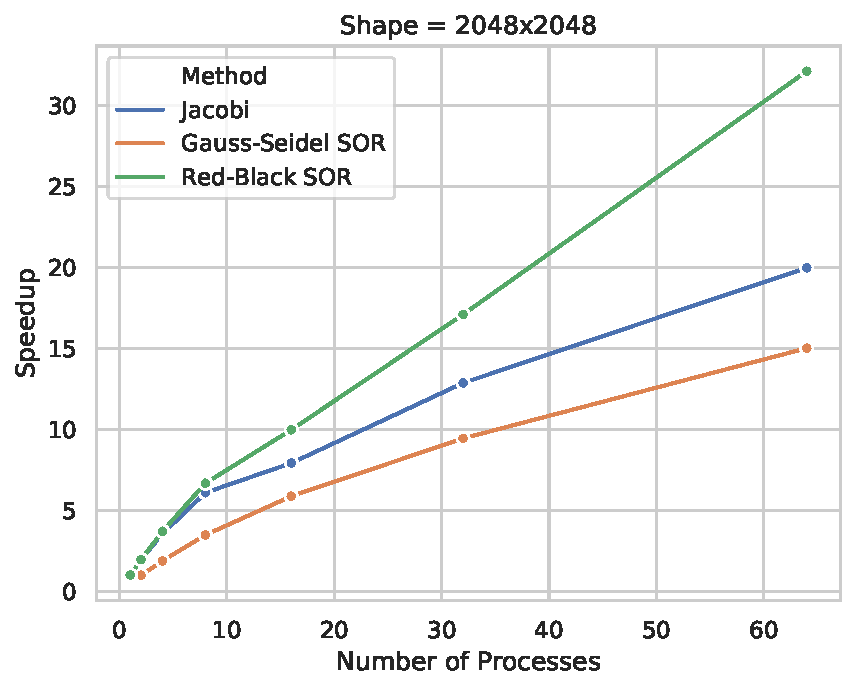
\includegraphics[width=0.49\textwidth]{speedup-2048x2048.pdf}
    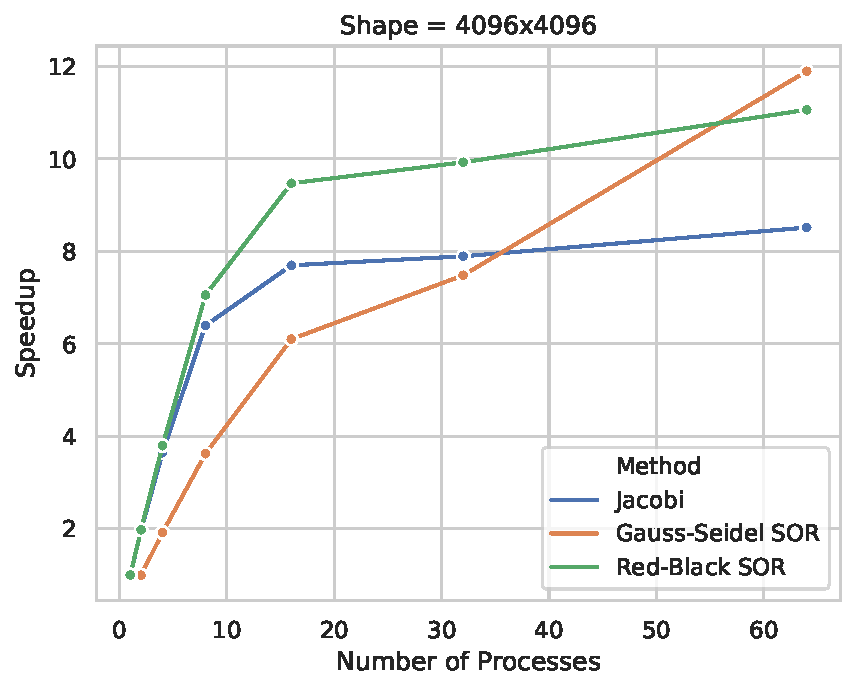
\includegraphics[width=0.49\textwidth]{speedup-4096x4096.pdf}
    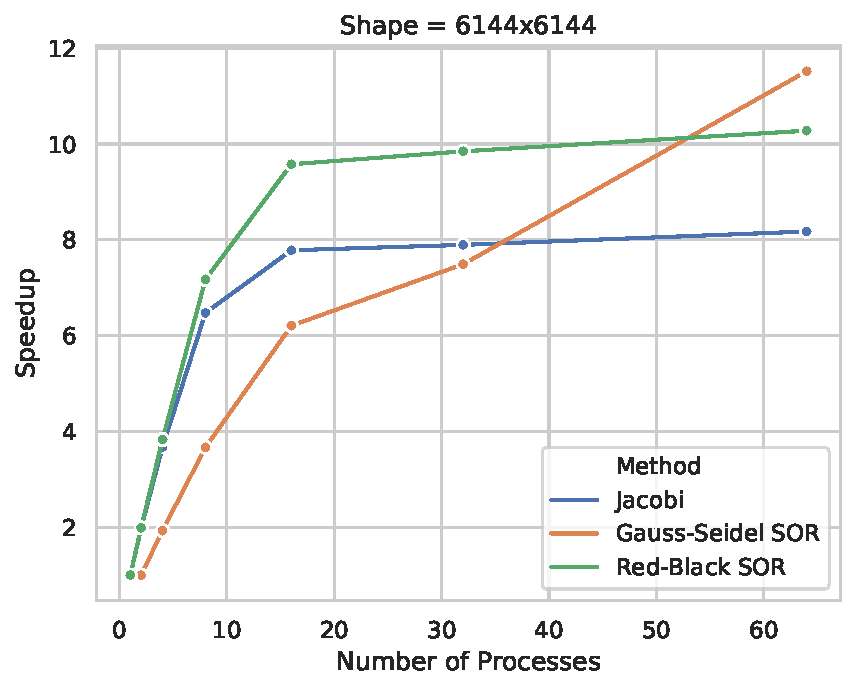
\includegraphics[width=0.49\textwidth]{speedup-6144x6144.pdf}
\end{center}

Παρατηρούμε ότι σταθερά ο Gauss-Seidel SOR έχει μικρότερο speedup από τον
Jacobi, που με τη σειρά του έχει χειρότερο speedup από τον Red-Black SOR.
Επίσης βλέπουμε ότι το speedup είναι πανομοιότυπο για τους δύο μεγάλους πίνακες
(εξαιρείται ο Red-Black SOR για 64 διεργασίες που εμφανίζει μια ελαφριά πτώση).
Ως εκ τούτου, θα σχολιάσουμε το speedup τους από κοινού.

Εστιάζοντας στο μικρό πίνακα παρατηρούμε για όλο το εύρος τιμών μια αύξηση του
speedup. Μάλιστα ο Jacobi και ο Red-Black SOR εμφανίζουν σχεδόν γραμμικό speedup
για έως και 8 διεργασίες, ενώ ο Red-Black SOR φαίνεται να αποκτά σημαντικό
προβάδισμα σε σχέση με τον Jacobi για περισσότερες διεργασίες.

Αντίθετα για τους μεγάλους πίνακες, παρότι το speedup φαίνεται να διατηρεί
όμοιες τιμές με το μικρό μέχρι και τις 16 διεργασίες, ο Jacobi και ο
Red-Black SOR εμφανίζουν έναν ξαφνικό κορεσμό για 32 και 64 διεργασίες.
Ωστόσο, ο Gauss-Seidel SOR, ενώ πράγματι χειροτερεύει λίγο, δεν φαίνεται να
κορέννυται. Έτσι καταλήγει να έχει καλύτερο speedup από τις υπόλοιπες
μεθόδους για 64 διεργασίες. Βέβαια το αποτέλεσμα αυτό είναι σχετικά
παραπλανητικό. Στην πραγματικότητα ο Gauss-Seidel SOR είχε ήδη μέτριο speedup,
οπότε τα αποτελέσματα του κορεσμού δεν του έγιναν αισθητά.

Αξίζει να σημειωθεί ότι η ομοιότητα μεταξύ Jacobi και Gauss-Seidel SOR εξηγείται
αν παρατηρήσουμε ότι εκτελούμε στην ουσία τον ίδιο αλγόριθμο σε 1 ή 2 φάσεις
αντίστοιχα.

Σε δεύτερη φάση κοιτάμε τους χρόνους εκτέλεσης και υπολογισμών. Για τον πίνακα
μεγέθους 2048x2048 έχουμε:

\begin{center}
    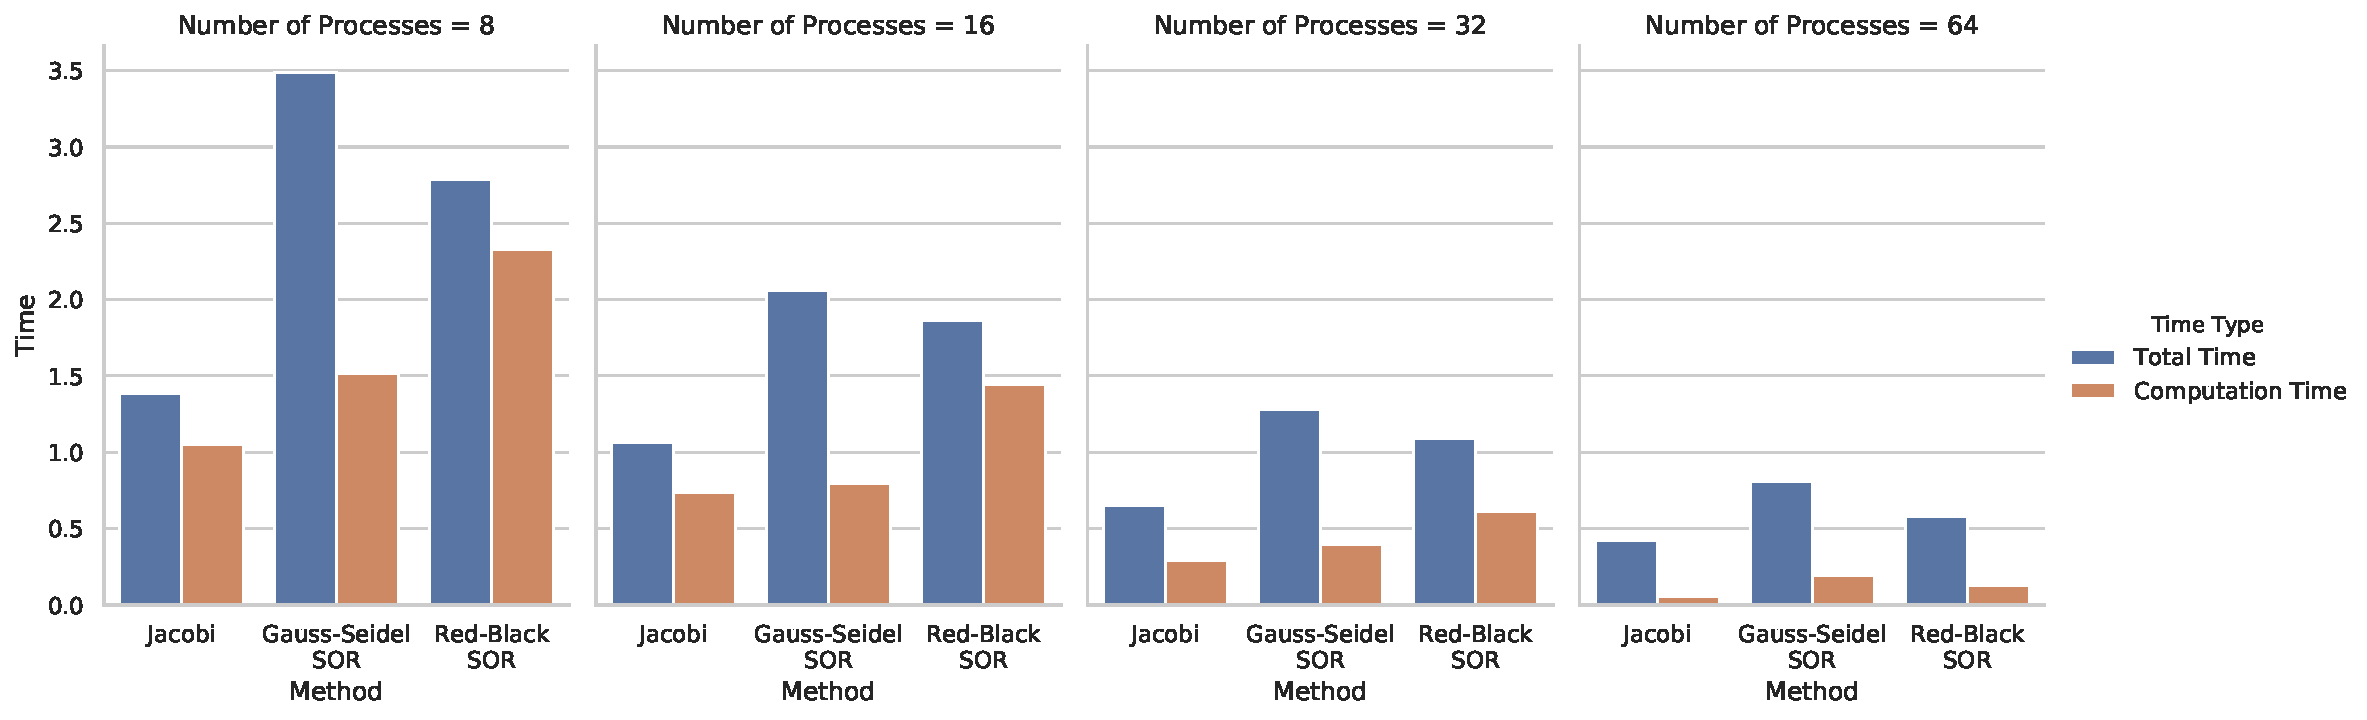
\includegraphics[width=1.15\textwidth]{time-2048x2048.pdf}
\end{center}

Ομοίως για τον πίνακα μεγέθους 4096x4096 έχουμε:

\begin{center}
    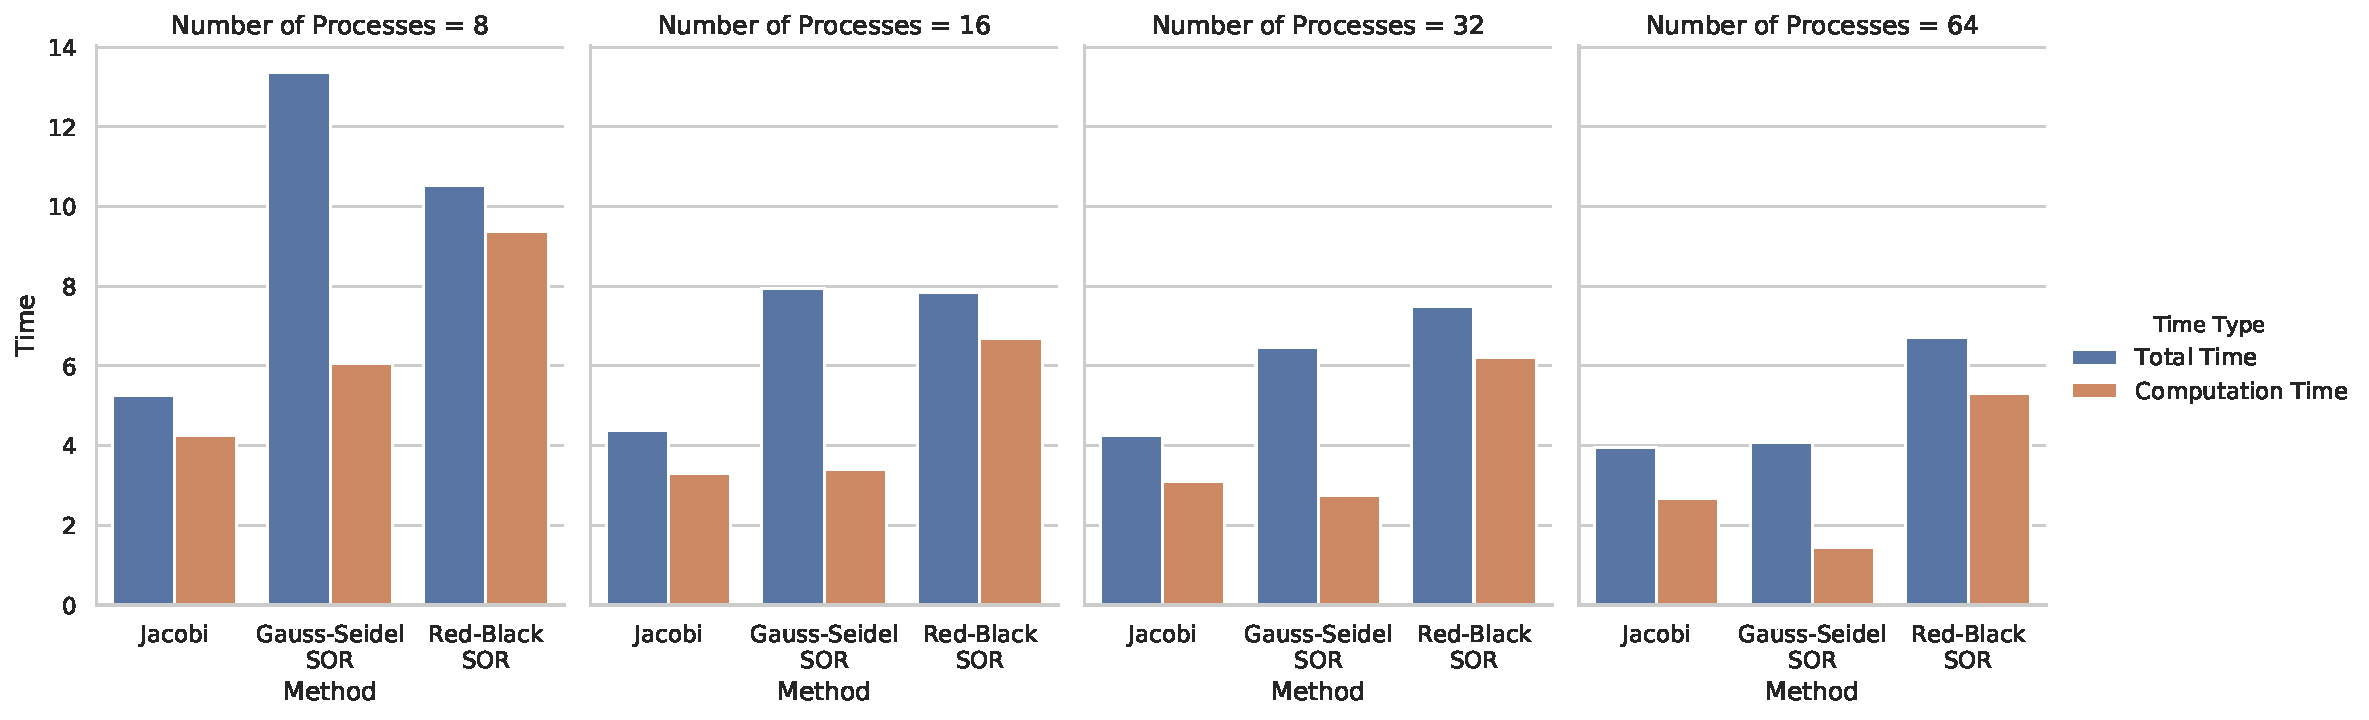
\includegraphics[width=1.15\textwidth]{time-4096x4096.pdf}
\end{center}

Τέλος για τον πίνακα μεγέθους 6144x6144 έχουμε:

\begin{center}
    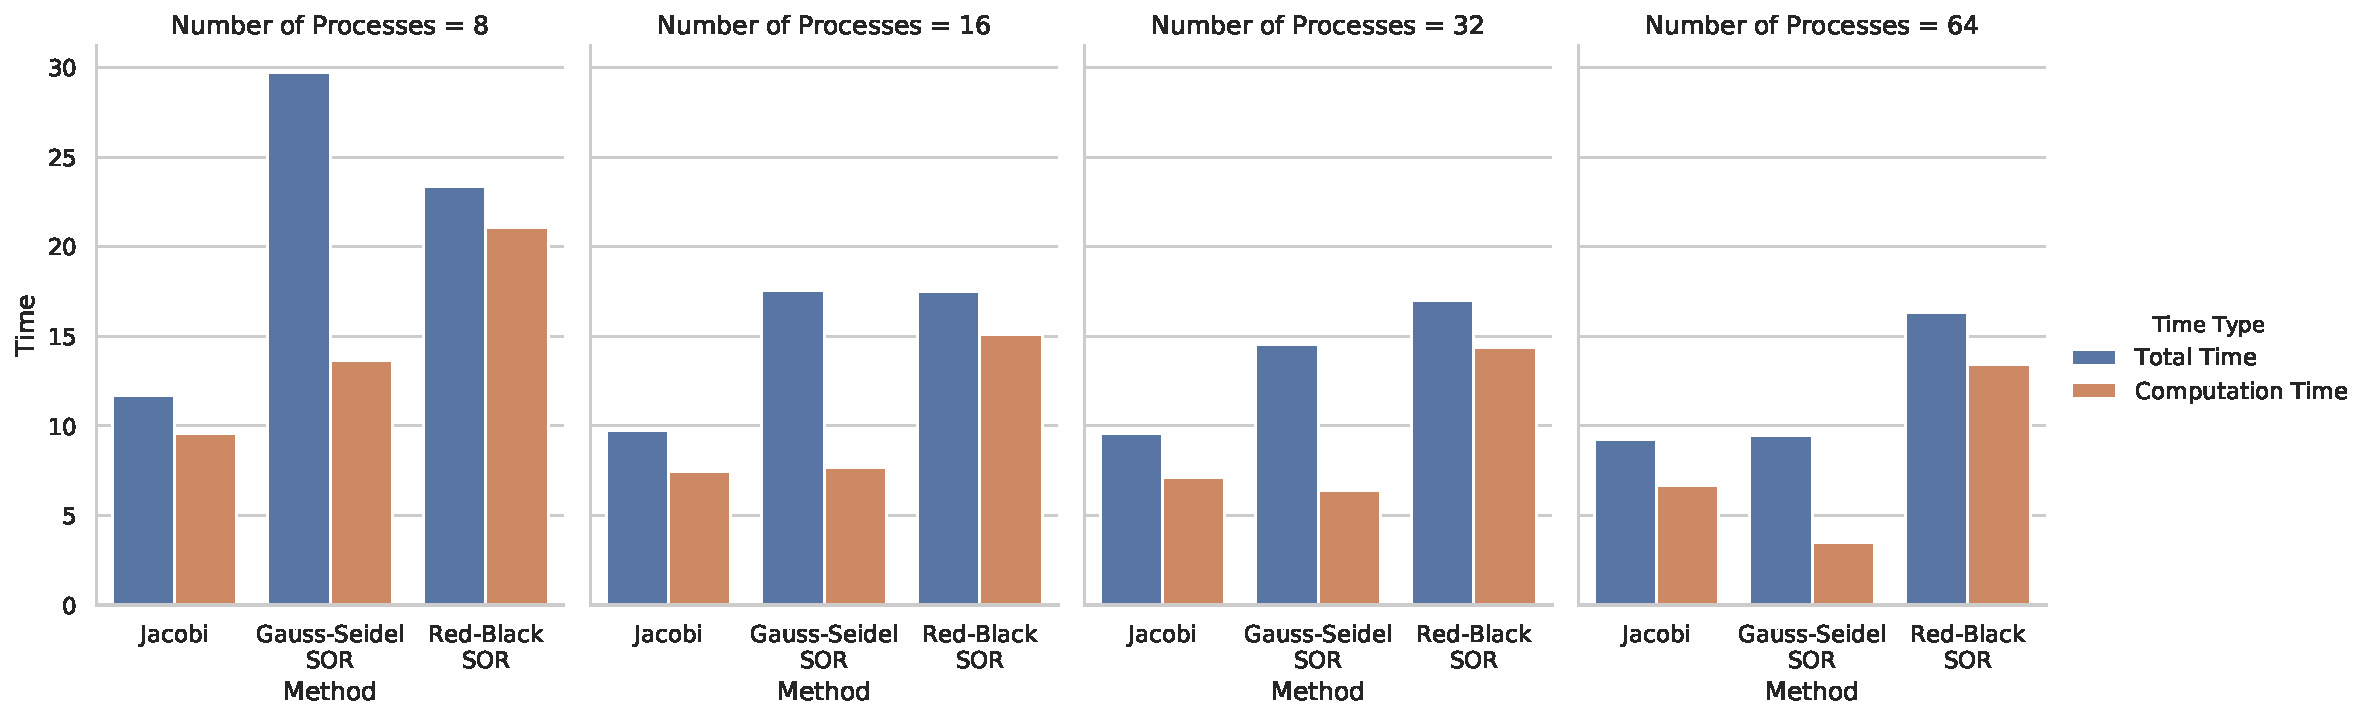
\includegraphics[width=1.15\textwidth]{time-6144x6144.pdf}
\end{center}

Αρχικά παρατηρούμε πάλι ότι η μορφή των διαγραμμάτων είναι ακριβώς η ίδια για
τους μεγάλους πίνακες. Ωστόσο, σε απόλυτα μεγέθη είναι αισθητή (και αναμενόμενη)
η διαφορά στους χρόνους.

Όσον αφορά τους χρόνους υπολογισμού, εύκολα βλέπουμε ότι για το μικρό πίνακα
εμφανίζουν μια σημαντική πτώση με την αύξηση του πλήθους των διεργασιών (ο
Red-Black SOR βελτιώνεται τόσο γρήγορα που για 64 διεργασίες έχει μικρότερο
χρόνο υπολογισμού από τον Gauss-Seidel SOR). Για το μεγάλο πίνακα η βελτίωση
μειώνεται αισθητά για 16 διεργασίες και άνω. Πάλι εξαιρείται ο Gauss-Seidel SOR
που συνεχίζει σταθερά να βελτιώνεται, καταφέρνοντας να ξεπεράσει στο χρόνο
υπολογισμού τις άλλες μεθόδους.

Παρόμοια τάση παρατηρούμε και στους συνολικούς χρόνους. Το ενδιαφέρον λοιπόν
βρίσκεται στον υπόλοιπο νεκρό χρόνο, που στην ουσία αποτελεί το χρόνο
επικοινωνίας. Είναι φανερό ότι ο χρόνος αυτός παραμένει πρακτικά σταθερός για
τον Jacobi και τον Red-Black SOR. Αντίθετα για τον Gauss-Seidel SOR, παρότι
είναι πάντα μεγαλύτερος από των άλλων, βλέπουμε μια συνεχή βελτίωσή του.

Πλέον βρισκόμαστε σε θέση να ερμηνεύσουμε τον κορεσμό που παρατηρήσαμε
προηγουμένως. Οι Jacobi και Red-Black SOR ακολουθούν ένα σχετικά απλό σχήμα
επικοινωνίας, κατά το οποίο εκτελούν όλους τους υπολογισμούς τους για μια
επανάληψη ή φάση αντίστοιχα και εν συνεχεία επικοινωνούν τα αποτελέσματά τους.
Ως αποτέλεσμα ο συγχρονισμός τους είναι σχετικά συγκεντρωμένος και απλός. Βέβαια 
αυτό σημαίνει ότι εκτελούνται ταυτόχρονα 8 ανταλλαγές μηνυμάτων μεταξύ κάθε
ζεύγους διεργασιών, γεγονός που οδηγεί εμφανώς σε bottleneck στο δίκτυο
διασύνδεσης.

Αντίθετα ο Gauss-Seidel SOR επιβάλλει έναν μικρό κύκλο αναμονής στην αρχή κάθε
επανάληψης και έναν μεγάλο κύκλο αναμονής στο τέλος της. Επομένως προξενεί μια
σειριοποίηση της επικοινωνίας, που είναι μάλιστα άνισα χωρισμένη. Ως εκ τούτου,
είναι αναμενόμενο να εμφανίζει το μεγαλύτερο χρόνο επικοινωνίας. Παράλληλα, ο
διαχωρισμός αυτός σημαίνει ότι μόλις 6 ανταλλαγές μηνυμάτων μπορεί να συμβούν
ταυτόχρονα, καθυστερώντας την εμφάνιση του bottleneck του δικτύου διασύνδεσης
και επιτρέποντας έτσι την αισθητή βελτίωση της (ήδη αργής) επικοινωνίας για
μεγαλύτερα πλήθη διεργασιών.

Αξιοσημείωτο είναι ότι ο Jacobi, που εμφανίζει τη χειρότερη σύκγλιση, καταλήγει
να είναι ο καλύτερος αλγόριθμος. Η βελτιστότητα αυτή οφείλεται προφανώς στην
απλότητά του. Δεν απαιτούνται ούτε 2 φάσεις που διπλασιάζουν τις ανάγκες
επικοινωνίας ούτε αναμονές και συγχρονισμοί πριν τους υπολογισμούς. Για σταθερό
αριθμό επαναλήψεων επομένως ο Jacobi καταλήγει να είναι ο (κίβδηλος) νικητής.

\end{document}